\documentclass{report}
\usepackage[utf8]{inputenc}

\title{Statistical Inference for Entropy}
\author{Karina Marks}

\usepackage{amsmath, amsfonts, graphicx, listings, booktabs, amstext, subcaption}
\usepackage[format=plain,
            textfont=it]{caption}
           


\newtheorem{theorem}{Theorem}
\newtheorem{remark}{Condition}

\begin{document}
\chapter{Conclusion}

As seen from the analysis undertaken in Chapter \ref{simulations-TODO}, taking an estimation of entropy from samples of the normal, uniform and exponential distributions, appear to act differently. There is no conclusive answer, that agrees across all three distributions,  as for the best value of $k$ for the estimator, or if the bias of the estimator is of $O \left( \frac{1}{N^{a}} \right)$ or $O\left( \left( \frac{k}{N} \right)^{a} \right)$. 

I wish to consider the optimal choice for the value of $k$, where I mean optimal in terms of reducing the bias, so the estimated value is as close to the exact value as possible. To do this, I have taken 1000 samples around the sample sizes of $500$, $10,000$, $20,000$, $30,000$, $40,000$ and $49,500$, found the average bias of the estimator for each $k$ and each distribution. I have graphically represented this in Figure \ref{OptimalK_graphs}. 

\begin{figure}
\makebox[\linewidth][c]{%
\begin{subfigure}[b]{.8\textwidth}
\centering
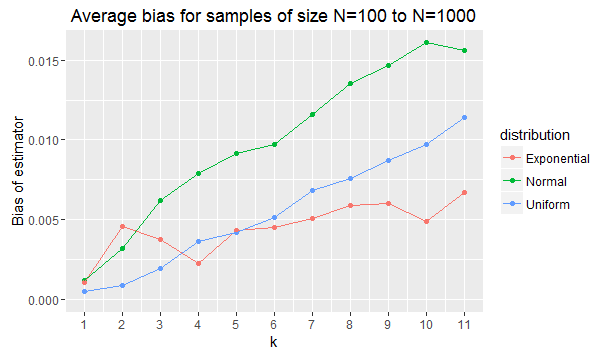
\includegraphics[width=\textwidth]{./Graphs/Best/kVbiasapprox100.png}
\caption{$N \approx 500$}
\end{subfigure}%
\begin{subfigure}[b]{.8\textwidth}
\centering
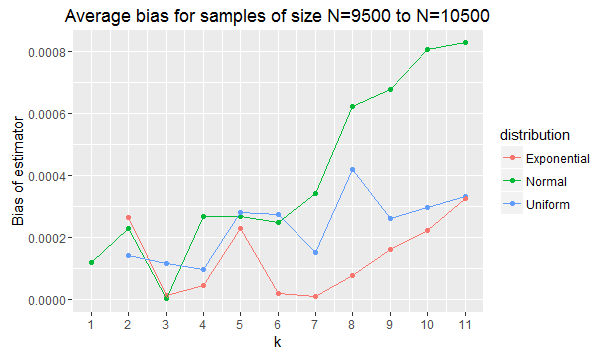
\includegraphics[width=\textwidth]{./Graphs/Best/kVbiasapprox10000.png}
\caption{$N \approx 10,000$}
\end{subfigure}%
}\    \makebox[\linewidth][c]{%
\begin{subfigure}[b]{.8\textwidth}
\centering
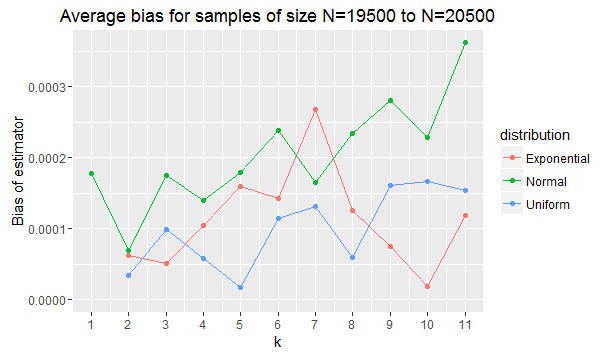
\includegraphics[width=\textwidth]{./Graphs/Best/kVbiasapprox20000.png}
\caption{$N \approx 20,000$}
\end{subfigure}%
\begin{subfigure}[b]{.8\textwidth}
\centering
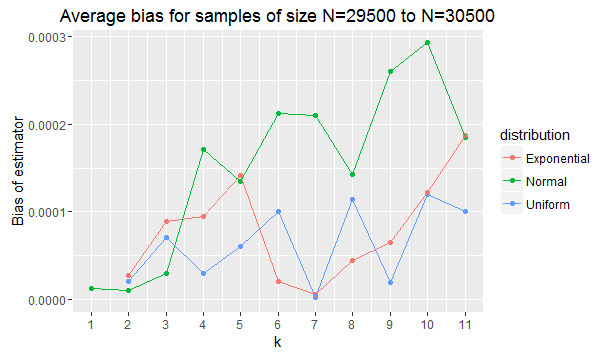
\includegraphics[width=\textwidth]{./Graphs/Best/kVbiasapprox30000.png}
\caption{$N \approx 30,000$}
\end{subfigure}%
}\    \makebox[\linewidth][c]{%
\begin{subfigure}[b]{.8\textwidth}
\centering
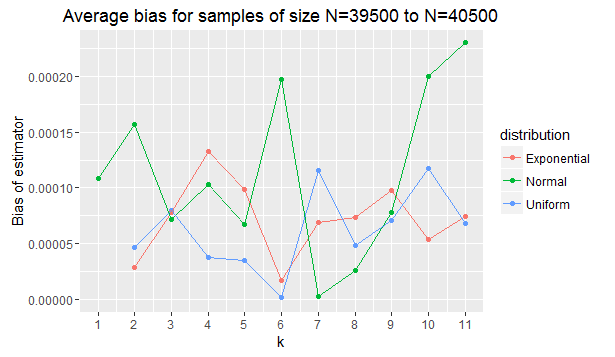
\includegraphics[width=\textwidth]{./Graphs/Best/kVbiasapprox40000.png}
\caption{$N \approx 40,000$}
\end{subfigure}%
\begin{subfigure}[b]{.8\textwidth}
\centering
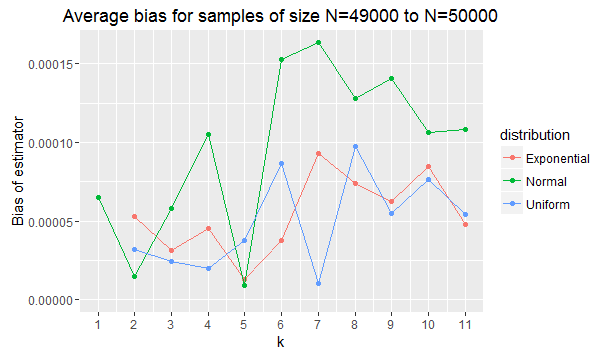
\includegraphics[width=\textwidth]{./Graphs/Best/kVbiasapprox50000.png}
\caption{$N \approx 49,500$}
\end{subfigure}%
}
\caption{TODO} \label{OptimalK_graphs}
\end{figure}


If we ignore the distribution, there is not an always obvious best value of $k$ shown by the graphs. Moreover, considering the analysis completed in section \ref{N_conditions}, we found that the values of $k$ that satisfy Theorems \ref{unbias} and \ref{efficient}, depend on $N$ so that $k \in \{k_{0}^{*}, ..., k_{1}^{*}\}$, where $k_{0}^{*} \approx 1$ and $k_{1}^{*} = O(N^{\frac{2}{9}})$. Thus for the samples in the graphs above, we can create a table of the values of $k$ that satisfy the conditions to be able to assume consistency and unbias of the estimator, Table \ref{ConditionK}.

\begin{table}
\caption{Values of $k$ satisfying Theorems \ref{efficient} and \ref{unbias} for sample sizes $N$} \label{ConditionK}
\begin{center}
\begin{tabular}{| l | c |} 
\toprule
N &  $k$ \\
\midrule[1pt]
$500$ & $\{1, 2, 3\}$ \\
$1,000$ & $\{1,2, 3, 4 \}$ \\
$10,000$ & $\{1, 2, ..., 7\}$ \\
$20,000$ & $\{1, 2, ..., 9\}$ \\
$30,000$ & $\{1,2, ..., 9 \}$ \\
$40,000$ & $\{1, 2, ...,10 \}$ \\
$50,000$ & $\{1, 2,  ..., 11\}$ \\
\hline
\end{tabular}
\\[10pt]
\end{center}
\end{table}

Although, for samples of size $N \leq 1,000$, we can see that, quite obviously, the smallest bias occurs with an estimator found using $k=1$, and this is true for all the distributions, graph (a). We can also see uniform increase in the bias, against the size of $k$ for both the uniform and normal distributions; thus for $N \approx 500$ and $k \in \{1,2, 3\}$, the optimal estimator is definitely found using $k=1$.

Considering graph (b) for sample size $N \approx 10,000$, we have that the smallest values of bias occur when $k=3$ or $7$ for the exponential, $k=3$ for the normal and $k=4$ for the uniform distributions. This agrees with the information found when finding $k$ to satisfy condition \ref{A3} we have that for this sample size $k \in \{1, 2, ... , 7\}$. This also implies that the most accurate estimator for a sample of this size could be found when using $k =3$ (or possibly $4$), since for all three distributions, at these values of $k$, we do have some of the smallest sizes of bias.

For graph (c), with $N \approx 20,000$, we have a range of values for $k$ with the smallest bias, depending on the distribution; for the exponential $k=10$, the normal $k=2$ and uniform $k=5$. However, considering that for this sample size we must have $k \in \{1, 2, ..., 9\}$, the value of $k$ for the exponential distribution cannot be $k=10$ for the Theorems \ref{efficient} and \ref{unbias} to be satisfied; thus the next smallest bias occurs when $k=3$. Due to this, nothing conclusive can be said about the optimal value of $k$, although, we could draw the conclusion that for this sample size, the best $k$ is from the range $k = \{2, 3, 5\}$. However, when choosing the values of $k$ that satisfy condition \ref{A3}, I made some approximations, which depended on the choice of $\alpha > d = 1$, and a value $\tau$ which is smaller than a bound. Due to this, the value of $tau$ could be chosen to be slightly larger; for example $\tau = \frac{19}{80} < \frac{1}{4}$, which would give $k_{1}^{*} = N^{\frac{19}{80}} = 20000^{\frac{19}{80}} = 10.507$. So $k=10$ could be included in the values that satisfy the Theorems and cannot be discounted. In fact, if we did use this new value of $\tau$, then the values for the optimum $k$ would be $k = \{2, 5, 10\}$, which makes even less sense. Thus, for this sample size we cannot draw any conclusions about the optimal value of $k$.

When $N \approx 30,000$, graph (d), we have the optimal values of $k$ - when the smallest bias occurs - being $2$ for the normal distribution and $7$ for both the uniform and exponential distributions. Interestingly, for all three distributions $k=2$ has either the first, second or third smallest bias, out of all $k$ for its own distribution. However, while the normal distribution has a general increase for $k > 2$, the other two distributions later dip to their lowest value of bias at $k=7$. Thus, while one may say that $k=7$ is the optimal, since it agrees with two of the three distributions, for the third distribution, the normal distribution, the bias is significantly higher. Henceforth, I would actually assume that a safer option, for the best value of $k$ across any distribution would be when $k=2$, where the bias for all three distributions is significantly small. All these values fit within those found in Table \ref{ConditionK}, and although $k = \{2, 7\}$ look to be the optimal values, no conclusion can be drawn for this value of $N$.

Now, for the graph (e), when $N \approx 40,000$ we have the smallest bias occurring at $k=6$ for the uniform and exponential and $k=7$ for the normal. If we consider the value for the bias at $k=6$ for the normal, we can see sudden significant increase in the size of the bias and a massive drop between this value, and that for $k=7$. Moreover, considering $k=7$ for the uniform and exponential distributions, we can see a substantial increase from the bias at $k=6$. Indicating, that the best value of $k$ may be $6$ or $7$; but this strongly depends on the distribution that the sample is taken from, not just the sample size. 

Lastly, for the final graph (f) with sample size $N \approx 50,000$, we can see that instead of the uniform and exponential agreeing as before, we now have the normal and exponential agreeing on its minimum value of bias at $k=5$, and the uniform minimum occurring at $k=7$. For the uniform distribution, the estimator with $k=5$ still holds a small bias, but there are four other values of $k$ with smaller bias for this distribution. For the normal distribution, there is a large jump at $k=7$, where the bias is much larger than before, and the exponential also shows a substantial jump. Thus, I would possibly agree that $k=5$ is the optimum choice for this sample size, but this result is not certain for all distributions. 

By considering all the information found from the graphs in Figure \ref{OptimalK_graphs}, for small sample sizes $N \leq 1,000$ we can say that $k=1$ would possibly be the best choice for $k$. However, I don't think anything conclusive can be drawn about a general distribution from a larger sample size $N$, despite some of the deductions above, there is no definitive choice for $k$ being obviously shown throughout each distribution considered. 

Perhaps an interesting graph to look at is that depicted in Figure \ref{k_bias_allN}, where I have taken all the data for every sample size $100 \leq N \leq 50,000$ and averaged the bias per distribution. I have done this to see if there is a safe value of $k$ to choose when wanting the estimator of entropy from a random sample to have the smallest bias.

\begin{figure}
  \begin{center}
    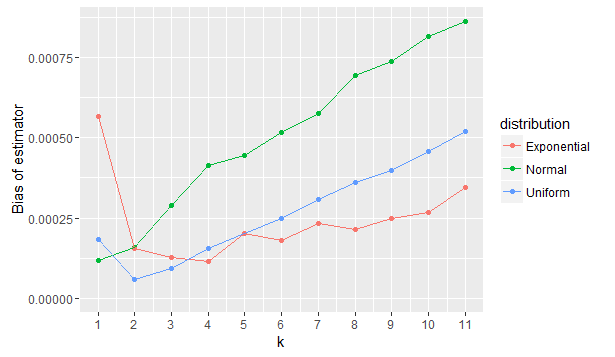
\includegraphics[width=\textwidth]{./Graphs/Best/kVbiasapproxALLN.png}
  \end{center}
\caption{ TODO }
  \label{k_bias_allN}
\end{figure}

From this, we can see that for a sample distributed like the normal, the safest value of $k$ to choose for any sample size is $k=1$, since on average, this gives the smallest bias of $\approx 0.000125$, regardless of its sample size. Then for all other values of $k$, the bias of the estimator increases with $k$; hence, if in doubt, I would recommend choosing $k=1$ if you suspect your 1-dimensional data to be normally distributed.

Considering the uniform distribution, we can see that the smallest average bias occurs at $k=2$, with the same behaviour as the normal for $k \geq 3$, whereby the bias increases with $k$. The average bias at $k=2$ is $\approx 0.0000625$, which is about half the size of that for the normal distribution. However, even though the relative size of the bias within a distribution is important to look at, the size between distributions is not as informative, due to the variability of the samples. Where for the normal distribution we have variance $\sigma^2 = 1$ and for the uniform we have variance $\frac{12}{100^2} = 0.0012$, which is significantly smaller - so we would expect a more accurate estimator due to this. Thus, when uncertain of which $k$ to choose, if the 1-dimensional data appears to be uniformly distributed, then it seems to be that $k=2$ would be the bes choice.

Lastly, looking at the most interesting result shown, those of the exponential distribution, which shows that, on average, the smallest bias occurs when $k=4$, with the bias generally increasing on both sides as $k$ increases/decreases away from $4$. The bias here is $\approx 0.000125$ - similar to that of the normal distribution, which is surprising owing to the fact that the samples from the exponential distribution were taken with a variability of $\frac{1}{0.5^2} = 4$, which is four times larger than the variance of the samples from the normal distribution. This is something very interesting about the exponential distribution, and I have noticed throughout my analysis that samples from this distribution do indeed act quite differently to those from the other two.

Another important aim of this paper was to consider whether the distributions imply the bias is of equations \ref{fixedkbias} or \ref{dependentkbias}; thus, whether bias is of $O \left( \frac{1}{N^{a}} \right)$ or $O\left( \left( \frac{k}{N} \right)^{a} \right)$. From the previous section, namely Figures \ref{c_k_normal}, \ref{c_k_uniform} and \ref{c_k_expo}, implied the following behaviours for the distributions considered, Table \ref{distribution_comparison}.

\begin{table}
\caption{Suspected behaviour of $Bias |\hat{H}_{N, k} |$ for each distribution} \label{distribution_comparison}
\begin{center}
\begin{tabular}{| c | c | c|} 
\toprule
Normal, $N(0,1)$ & Uniform, $U[0,100]$ & Exponential, $exp(0.5)$ \\
\midrule[1pt]
$O\left( \left( \frac{k}{N} \right)^{a} \right)$ & $O\left( \left( \frac{k}{N} \right)^{a} \right)$ &  $O \left( \frac{1}{N^{a}} \right)$ \\
\hline
\end{tabular}
\\[10pt]
\end{center}
\end{table}



TODO - check the values of $k$ maybe there is more that one?

difference in which k is best

difference in the order of the bias










\end{document}